%%%%%%%%%%%%%%%%%%%%%%%%%%%%%%%%%%%%%%%%%%%%%%%%%%%%%%%%%%%%%%%
% Course introduction
% Machine Learning : overview
% Learn from data: an output from an input, a decision, a representation, ...
% The main tasks in ML 
% Deep learning and feature ing.
%%%%%%%%%%%%%%%%%%%%%%%%%%%%%%%%%%%%%%%%%%%%%%%%%%%%%%%%%%%%%%%
\begin{frame}{Starter: a ``simple'' question}
  \framesubtitle{What it is ?}
    \begin{columns}
      \column{0.3\textwidth} %%%%%%%%%%%%%%%%%
      \begin{center}
        \includegraphics[width=\textwidth]{../figs/dog_drawing}
        \\[3ex]\pause
        \includegraphics[width=\textwidth]{../figs/dog-sad}\pause
      \end{center}
      \column{0.6\textwidth} %%%%%%%%%%%%%%%%%

      \begin{block}{Can you write an algorithm to answer ?}
        \pause
        \begin{itemize}
        \item What is the input space ? 
        \item What do you want to predict ? \\  human generated ? resolution ? 
          real ? outdoor ? the type of dogs ?
        \item The output space ? (binary, multi-class, regression)
        \end{itemize}
      \end{block}
      \begin{block}{And then ?}
        \pause
        \begin{itemize}
        \item What are the features ? 
        \item The decision rule ? 
        \item The evaluation criterion ? 
        \end{itemize}
      \end{block}
    \end{columns}
  \end{frame}

  
%%%%%%%%%%%%%%%%%%%%%%%%%%%%%%%%%%%%%%%%%%%%%%%%%%%%%%%%%%%%%%%
\begin{frame}{Starter: a less ``simple'' question}
    \begin{columns}
      \column{0.3\textwidth} %%%%%%%%%%%%%%%%%
      \begin{center}
        \includegraphics[width=\textwidth]{../figs/object_detection}
      \end{center}
      \column{0.6\textwidth} %%%%%%%%%%%%%%%%%
      \begin{block}{Can you write an algorithm to answer ? }
        \begin{itemize}
        \item What is the input space ? 
        \item What do you want to predict ? \\  a set of tagged bounding boxes
        \item The output space ?\\ multi-class depending on the application
        \end{itemize}
      \end{block}
      \begin{block}{And then ?}
      \pause
      \begin{itemize}
      \item Two tasks: segmentation and classification (joint)
      \item What are the features ? 
      \item The decision rule ?
      \item The evaluation criterion ? 
      \end{itemize}
    \end{block}
    \end{columns}
  \end{frame}

%%%%%%%%%%%%%%%%%%%%%%%%%%%%%%%%%%%%%%%%%%%%%%%%%%%%%%%%%%%%%%%
\begin{frame}{Starter: a less ``simple'' question}
  \framesubtitle{Named Entity Recognition (NER)}
  \begin{columns}
      \column{0.65\textwidth} %%%%%%%%%%%%%%%%%
      \begin{center}
        \includegraphics[width=\textwidth]{../figs/ner}
      \end{center}
      \column{0.35\textwidth} %%%%%%%%%%%%%%%%%
      Can you write an algorithm ?
      % Just gather list of NE but it is not enough
      % language is ambiguous (e.g. Tim Cook)
      % language is evolving (new TV star, new places, new language of interest, ...)
      % answer is obvious (most of the time), but hard to explain
      \begin{itemize}
      \item The input space ? 
      \item The prediction ? \\  %tagged text segments 
      \item The output space ?\\ %multi-class depending on the application
      \end{itemize}
    \end{columns}\pause
    \begin{block}{Just build lists of Named entities ?} 
      \begin{itemize}
      \item language is ambiguous (e.g. Tim Cook, 1984, ... )
      \item language is evolving with new ``people'', places, domain specific terms, ...
      \item answer is obvious (most of the time), but hard to explain
     \end{itemize}
  \end{block}
\end{frame}


%%%%%%%%%%%%%%%%%%%%%%%%%%%%%%%%%%%%%%%%%%%%%%%%%%%%%%%%%%%%%%%
\begin{frame}{The Machine Learning way}
\framesubtitle{How to make a ‘computer’ do a specific task?}
\begin{block}{Traditional approach (old AI)}
A program is:
\begin{itemize}
\item hand-coded
\item specific set of instructions to complete the task
\item can be explained and proved, ``always'' gives the correct answer
\end{itemize}
\end{block}


% The inductive bias (also known as learning bias) of a learning
% algorithm is the set of assumptions that the learner uses to predict
% outputs given inputs that it has not encountered.[1]

% In machine learning, one aims to construct algorithms that are able
% to learn to predict a certain target output. To achieve this, the
% learning algorithm is presented some training examples that
% demonstrate the intended relation of input and output values. Then
% the learner is supposed to approximate the correct output, even for
% examples that have not been shown during training. Without any
% additional assumptions, this problem cannot be solved exactly since
% unseen situations might have an arbitrary output value. The kind of
% necessary assumptions about the nature of the target function are
% subsumed in the phrase inductive bias.

% A classical example of an inductive bias is Occam's razor, assuming
% that the simplest consistent hypothesis about the target function is
% actually the best. Here consistent means that the hypothesis of the
% learner yields correct outputs for all of the examples that have
% been given to the algorithm.
\begin{block}{Machine Learning}
A program is:
\begin{itemize}
\item trained or learnt 
\item from large amount of annotated data 
\item algorithm + inductive bias
\item it works ... on average
\end{itemize}
\end{block}
\end{frame}



\begin{frame}{Machine learning: the main tasks}
  \framesubtitle{Supervised classification}
  \begin{center}
    \tikz[baseline=0]{ \node at (-2,0)
      {\includegraphics[height=0.25\textheight]{figs/mnist_5.pdf}}; %
      \node at (-0.4,0) {:}; \xvector{0}{-0.75}{6} }
    $\x \in \real^{784} \ \longrightarrow \class  \in\{0, 1,2, \ldots ,9
    \}$
  \end{center}
  \begin{itemize}
  \item $\dataset= (\exi , \classi )_{i=1}^{\nsamples}$ 
  \item \important{Supervised} learning of a \important{classification} task
  \end{itemize}
\end{frame}

\begin{frame}{Machine learning: the main tasks}
  \framesubtitle{Supervised binary classification}
  \begin{center}
    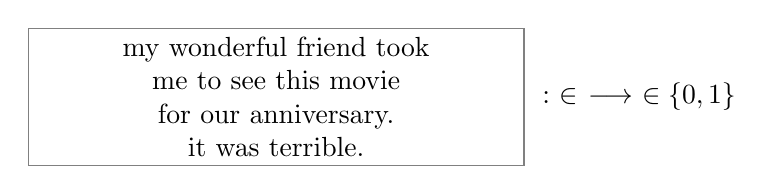
\begin{tikzpicture}
        %%%%%%%%%%%%%%%%%%%%%
      \node[anchor=east,draw=gray,text width=0.5\textwidth,align=center] (review) at
      (0,0) {my wonderful friend took me to see this movie \\for our
        anniversary. \\ it was terrible.};
      %%%%%%%%%%%%%%%%%%%%%
      \node[anchor=west] (txt) at (0.1,0) {$: \ \x \in \real^{\nfeats} \ \longrightarrow \ \class \in\{0, 1\}$};
    \end{tikzpicture}
  \end{center}

  \begin{itemize}
  \item $\dataset= (\exi , \classi )_{i=1}^{\nsamples}$ 
  \item Supervised learning of a \important{binary} classification task
  \end{itemize}

\end{frame}


\begin{frame}{Machine learning: the main tasks}
  \framesubtitle{Supervised regression}
  \begin{center}
    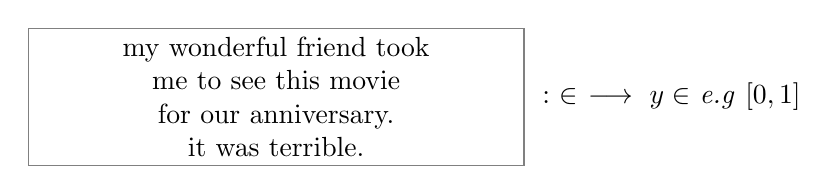
\begin{tikzpicture}
      %%%%%%%%%%%%%%%%%%%%% 
      \node[anchor=east,draw=gray,text width=0.5\textwidth,align=center] (review) at
      (0,0) {my wonderful friend took me to see this movie \\for our
        anniversary. \\ it was terrible.};
      %%%%%%%%%%%%%%%%%%%%%
      \node[anchor=west] (txt) at (0.1,0) {$: \ \x \in \real^{\nfeats}
        \ \longrightarrow \ y \in \real$ \textit{e.g} $[0, 1]$ };
    \end{tikzpicture}
  \end{center}

  \begin{itemize}
  \item $\dataset= (\exi, {\y}\sid{i})_{i=1}^{\nsamples}$ 
  \item Supervised learning of a \important{regression} task
  \end{itemize}
\end{frame}



\begin{frame}{Machine learning: the main tasks}
  \framesubtitle{Unsupervised learning / Clustering}
  \begin{columns}
    \column{0.45\textwidth}
    \begin{figure}[htb]
      \centerline{
%        \includegraphics[height = 0.6\textheight]{book_pile}
        \scalebox{0.15}{\includegraphics{../figs/book_pile}}
      }
    \end{figure}
    \column{0.1\textwidth}
    \begin{Huge}
    $\Longrightarrow$
    \end{Huge}
    \column{0.45\textwidth}
    \begin{figure}[htb]
      \centerline{
        \scalebox{0.3}{\includegraphics{../figs/book_clusters}}
      }
    \end{figure}
  \end{columns}
  $$ \x \in \real^{\nfeats} \ \longrightarrow \ \seq{z} \in \real^{\nclasses}$$
  \begin{itemize}
  \item A set of observations $\dataset= (\exi)_{i=1}^{\nsamples}$ must be assigned to a cluster $\rightarrow z$
  \item The model infer a hidden/latent structure in the $\dataset$ 
  \item The \textit{guidelines}: the structure of the model, the assumptions (distance, similarty between the $\x$, ... )
  \item Dimensionality reduction, data mining, ... 
  \end{itemize}
\end{frame}

  
\begin{frame}{Machine learning: the main tasks}
  \framesubtitle{Unsupervised learning}
  \begin{center}
    \begin{tikzpicture}
      \node at (0,0)
      {\includegraphics[height=0.4\textheight]{figs/lda.pdf}}; 
        %%%%%%%%%%%%%%%%%%%%%
      \node[anchor=west] (txt) at (4,0) {$: \ \exi \in \real^{\nfeats}
        \ \longrightarrow \ \seq{z} \in \real^{d}$};
    \end{tikzpicture}
  \end{center}

  \begin{itemize}
  \item $\dataset= (\exi )_{i=1}^{\nsamples} \longrightarrow (\seq{z}\sid{i})$, the outcome of the learning algorithm
  \item \important{Unsupervised} learning 
  \end{itemize}
  (K-means, GMM, LDA, ... )
\end{frame}





\begin{frame}
  \frametitle{Feature engineering}
  \begin{center}
    Most current machine learning works well because of
    human-designed representations and input features\\[1cm]
    {\includegraphics[height=0.4\textheight]{./figs/ml_2.pdf}}
    \begin{itemize}
    \item Time consuming and task/domain dependant
    \item Features are often both over-specified and incomplete
    \item Machine learning $\Leftrightarrow$ optimizing parameters to 
      make the best prediction
    \end{itemize}
  \end{center}
\end{frame}

\begin{frame}
  \frametitle{Representation learning and Deep networks}
  \begin{center}
    Representation learning attempts to
    automatically learn useful features\\[1cm]
    {\includegraphics[height=0.4\textheight]{./figs/ml_3.pdf}}
  \end{center}
  \begin{itemize}
  \item Learning a hierarchical and abstract representation
  \item That can be shared among tasks
  \item Almost all data is unlabeled $\Rightarrow$ unsupervised learning
  \end{itemize}
\end{frame}


\begin{frame}
  \frametitle{Neural Networks}
  \begin{center}
    \includegraphics[width=0.7\textwidth]{./figs/deeplearning}
    \scriptsize{(from Bengio, 2015)}
  \end{center}
\end{frame}



\begin{frame}
  \frametitle{Illustration}
  \begin{center}
    \includegraphics[height=0.75\textheight]{./figs/face_features}
  \end{center}
  \begin{flushright}
    \cite{Lee09convDBN}
  \end{flushright}
\end{frame}



\begin{frame}{Deep learning in neural networks : a  success story}
  \begin{columns}
    \column{0.6\textwidth}
    \begin{block}{Since 2009, deep learning approaches won several challenges}
    \begin{itemize}
    \item ImageNet since 2012 \cite{Krizhevsky12ImageNet} 
    \item Traffic signs recognition: superhuman performance in 2011 \cite{Ciresan12Multicolumn} based on \cite{LeCun89}
    \item Handwritting recognition since 2009 \cite{Graves09Offline} based on \cite{Hochreiter97LSTM}
    \item Automatic Speech recognition \cite{Hinton12ASR}
    \item Machine translation \cite{Vaswani17Attention}
    \end{itemize}
  \end{block}
  \column{0.4\textwidth}
  \begin{center} 
      \includegraphics[width=0.6\textwidth]{./figs/trafficsigns}\\
     \includegraphics[width=0.8\textwidth]{./figs/ocr}
  \end{center}
\end{columns}
\end{frame}




\begin{frame}{Deep learning in neural networks: a  long story}
   \begin{block}{The breakthrough of 2006}
     The expression \emph{Deep Learning} was coined around 2006 with papers on unsupervised pre-training of neural nets~\cite{Hinton06Deep,Hinton06Science,Bengio07Greedy}
   \end{block}
   \begin{block}{And before ? (just a few dates)}
     \begin{itemize}
     \item 1958 Rosenblatt proposed the perceptron \cite{Rosenblatt58Perceptron}, following the work of McCulloch and Pitts in 1943 and Hebb in 1949. 
     \item 1980 Neocognitron \cite{Fukushima80Neocognitron} or the multilayered NNets
     \item 1982 Hopfield network with memory and recurrence \cite{Hopfield82Neural}, the unsupervised SOM \cite{Kohonen82SOM}, Neural PCA \cite{Oja82NeuralPCA}
%     \item 1985 Boltzmann machines (Ackley et al., 1985)
     \item 1986 Multilayer perceptrons and backpropagation \cite{Rumelhart86BP}
%     \item 1988 RBF networks (Broomhead Lowe, 1988)
     \item 1989 Autoencoders \cite{Baldi89AE}, Convolutional network \cite{LeCun89}
     \item 1993 Sparse coding \cite{Field93Sparse}
     \end{itemize}
   \end{block}
\end{frame}


\begin{frame}{What is new ?}
\framesubtitle{From Kyunghyun Cho's slides (2015)}
\begin{columns}
  \begin{column}{0.6\textwidth}
    \begin{block}{Why today ?}
      \begin{itemize}
      \item We have connected the dots, e.g. \\
        (Probabilistic) PCA / Neural PCA / Autoencoder
      \item We understand learning better (regularization,
        architecture)
      \item No need to be scared of non-convex optimization
        (initialization)
      \item  {\color{red} The huge amount of data and the growth of computational
        power.}
      \end{itemize}
    \end{block}
    \begin{block}{What is the difference between a NNet and a Deep
        Network ?}
      An (very) intensive empirical exploration of the different issues
    \end{block}
  \end{column}    
  %%%%%%%%%%%%%%%%%%%%%%%%%
  \begin{column}{0.4\textwidth}
    \includegraphics[width=1\textwidth]{./figs/deep_relu2}
{\vfill\footnotesize{Y. Bengio, 2015}}
  \end{column}
\end{columns}
\end{frame}

\begin{frame}
  \begin{center}
    \includegraphics[width=0.45\textwidth]{./figs/miracle2}\\
  \end{center}
\end{frame}
 
\endinput



